
\documentclass[letterpaper,hide notes,xcolor={table,svgnames},pdftex,10pt]{beamer}
\def\showexamples{t}


%\usepackage[svgnames]{xcolor}

%% Demo talk
%\documentclass[letterpaper,notes=show]{beamer}

\usecolortheme{crane}
\setbeamertemplate{navigation symbols}{}

\usetheme{MyPittsburgh}
%\usetheme{Frankfurt}

%\usepackage{tipa}

\usepackage{hyperref}
\usepackage{graphicx,xspace}
\usepackage[normalem]{ulem}
\usepackage{multicol}

\newcommand\SF[1]{$\bigstar$\footnote{SF: #1}}

\usepackage[default]{sourcesanspro}
\usepackage[T1]{fontenc}

\newcounter{tmpnumSlide}
\newcounter{tmpnumNote}

% old question code
%\newcommand\question[1]{{$\bigstar$ \small \onlySlide{2}{#1}}}
% \newcommand\nquestion[1]{\ifdefined \presentationonly \textcircled{?} \fi \note{\par{\Large \textbf{?}} #1}}
% \newcommand\nanswer[1]{\note{\par{\Large \textbf{A}} #1}}


 \newcommand\mnote[1]{%
   \addtocounter{tmpnumSlide}{1}
   \ifdefined\showcues {~\tiny\fbox{\arabic{tmpnumSlide}}}\fi
   \note{\setlength{\parskip}{1ex}\addtocounter{tmpnumNote}{1}\textbf{\Large \arabic{tmpnumNote}:} {#1\par}}}

\newcommand\mmnote[1]{\note{\setlength{\parskip}{1ex}#1\par}}

%\newcommand\mnote[2][]{\ifdefined\handoutwithnotes {~\tiny\fbox{#1}}\fi
% \note{\setlength{\parskip}{1ex}\textbf{\Large #1:} #2\par}}

%\newcommand\mnote[2][]{{\tiny\fbox{#1}} \note{\setlength{\parskip}{1ex}\textbf{\Large #1:} #2\par}}

\newcommand\mquestion[2]{{~\color{red}\fbox{?}}\note{\setlength{\parskip}{1ex}\par{\Large \textbf{?}} #1} \note{\setlength{\parskip}{1ex}\par{\Large \textbf{A}} #2\par}\ifdefined \presentationonly \pause \fi}

\newcommand\blackboard[1]{%
\ifdefined   \showblackboard
  {#1}
  \else {\begin{center} \fbox{\colorbox{blue!30}{%
         \begin{minipage}{.95\linewidth}%
           \hspace{\stretch{1}} Some space intentionally left blank; done at the blackboard.%
         \end{minipage}}}\end{center}}%
         \fi%
}



%\newcommand\q{\tikz \node[thick,color=black,shape=circle]{?};}
%\newcommand\q{\ifdefined \presentationonly \textcircled{?} \fi}

\usepackage{listings}
\lstset{%
  keywordstyle=\bfseries,
  aboveskip=15pt,
  belowskip=15pt,
  captionpos=b,
  identifierstyle=\ttfamily,
  escapeinside={(*@}{@*)},
  stringstyle=\ttfamiliy,
  frame=lines,
  numbers=left, basicstyle=\scriptsize, numberstyle=\tiny, stepnumber=0, numbersep=2pt}

\usepackage{siunitx}
\newcommand\sius[1]{\num[group-separator = {,}]{#1}\si{\micro\second}}
\newcommand\sims[1]{\num[group-separator = {,}]{#1}\si{\milli\second}}
\newcommand\sins[1]{\num[group-separator = {,}]{#1}\si{\nano\second}}
\sisetup{group-separator = {,}, group-digits = true}

%% -------------------- tikz --------------------
\usepackage{tikz}
\usetikzlibrary{positioning}
\usetikzlibrary{arrows,backgrounds,automata,decorations.shapes,decorations.pathmorphing,decorations.markings,decorations.text}

\tikzstyle{place}=[circle,draw=blue!50,fill=blue!20,thick, inner sep=0pt,minimum size=6mm]
\tikzstyle{transition}=[rectangle,draw=black!50,fill=black!20,thick, inner sep=0pt,minimum size=4mm]

\tikzstyle{block}=[rectangle,draw=black, thick, inner sep=5pt]
\tikzstyle{bullet}=[circle,draw=black, fill=black, thin, inner sep=2pt]

\tikzstyle{pre}=[<-,shorten <=1pt,>=stealth',semithick]
\tikzstyle{post}=[->,shorten >=1pt,>=stealth',semithick]
\tikzstyle{bi}=[<->,shorten >=1pt,shorten <=1pt, >=stealth',semithick]

\tikzstyle{mut}=[-,>=stealth',semithick]

\tikzstyle{treereset}=[dashed,->, shorten >=1pt,>=stealth',thin]

\usepackage{ifmtarg}
\usepackage{xifthen}
\makeatletter
% new counter to now which frame it is within the sequence
\newcounter{multiframecounter}
% initialize buffer for previously used frame title
\gdef\lastframetitle{\textit{undefined}}
% new environment for a multi-frame
\newenvironment{multiframe}[1][]{%
\ifthenelse{\isempty{#1}}{%
% if no frame title was set via optional parameter,
% only increase sequence counter by 1
\addtocounter{multiframecounter}{1}%
}{%
% new frame title has been provided, thus
% reset sequence counter to 1 and buffer frame title for later use
\setcounter{multiframecounter}{1}%
\gdef\lastframetitle{#1}%
}%
% start conventional frame environment and
% automatically set frame title followed by sequence counter
\begin{frame}%
\frametitle{\lastframetitle~{\normalfont(\arabic{multiframecounter})}}%
}{%
\end{frame}%
}
\makeatother

\makeatletter
\newdimen\tu@tmpa%
\newdimen\ydiffl%
\newdimen\xdiffl%
\newcommand\ydiff[2]{%
    \coordinate (tmpnamea) at (#1);%
    \coordinate (tmpnameb) at (#2);%
    \pgfextracty{\tu@tmpa}{\pgfpointanchor{tmpnamea}{center}}%
    \pgfextracty{\ydiffl}{\pgfpointanchor{tmpnameb}{center}}%
    \advance\ydiffl by -\tu@tmpa%
}
\newcommand\xdiff[2]{%
    \coordinate (tmpnamea) at (#1);%
    \coordinate (tmpnameb) at (#2);%
    \pgfextractx{\tu@tmpa}{\pgfpointanchor{tmpnamea}{center}}%
    \pgfextractx{\xdiffl}{\pgfpointanchor{tmpnameb}{center}}%
    \advance\xdiffl by -\tu@tmpa%
}
\makeatother
\newcommand{\copyrightbox}[3][r]{%
\begin{tikzpicture}%
\node[inner sep=0pt,minimum size=2em](ciimage){#2};
\usefont{OT1}{phv}{n}{n}\fontsize{4}{4}\selectfont
\ydiff{ciimage.south}{ciimage.north}
\xdiff{ciimage.west}{ciimage.east}
\ifthenelse{\equal{#1}{r}}{%
\node[inner sep=0pt,right=1ex of ciimage.south east,anchor=north west,rotate=90]%
{\raggedleft\color{black!50}\parbox{\the\ydiffl}{\raggedright{}#3}};%
}{%
\ifthenelse{\equal{#1}{l}}{%
\node[inner sep=0pt,right=1ex of ciimage.south west,anchor=south west,rotate=90]%
{\raggedleft\color{black!50}\parbox{\the\ydiffl}{\raggedright{}#3}};%
}{%
\node[inner sep=0pt,below=1ex of ciimage.south west,anchor=north west]%
{\raggedleft\color{black!50}\parbox{\the\xdiffl}{\raggedright{}#3}};%
}
}
\end{tikzpicture}
}


%% --------------------

%\usepackage[excludeor]{everyhook}
%\PushPreHook{par}{\setbox0=\lastbox\llap{MUH}}\box0}

%\vspace*{\stretch{1}

%\setbox0=\lastbox \llap{\textbullet\enskip}\box0}

\setlength{\parskip}{\fill}

\newcommand\noskips{\setlength{\parskip}{1ex}}
\newcommand\doskips{\setlength{\parskip}{\fill}}

\newcommand\xx{\par\vspace*{\stretch{1}}\par}
\newcommand\xxs{\par\vspace*{2ex}\par}
\newcommand\tuple[1]{\langle #1 \rangle}
\newcommand\code[1]{{\sf \footnotesize #1}}
\newcommand\ex[1]{\uline{Example:} \ifdefined \presentationonly \pause \fi
  \ifdefined\showexamples#1\xspace\else{\uline{\hspace*{2cm}}}\fi}

\newcommand\ceil[1]{\lceil #1 \rceil}


\AtBeginSection[]
{
   \begin{frame}
       \frametitle{Outline}
       \tableofcontents[currentsection]
   \end{frame}
}



\pgfdeclarelayer{edgelayer}
\pgfdeclarelayer{nodelayer}
\pgfsetlayers{edgelayer,nodelayer,main}

\tikzstyle{none}=[inner sep=0pt]
\tikzstyle{rn}=[circle,fill=Red,draw=Black,line width=0.8 pt]
\tikzstyle{gn}=[circle,fill=Lime,draw=Black,line width=0.8 pt]
\tikzstyle{yn}=[circle,fill=Yellow,draw=Black,line width=0.8 pt]
\tikzstyle{empty}=[circle,fill=White,draw=Black]
\tikzstyle{bw} = [rectangle, draw, fill=blue!20, 
    text width=4em, text centered, rounded corners, minimum height=2em]
    
    \newcommand{\CcNote}[1]{% longname
	This work is licensed under the \textit{Creative Commons #1 3.0 License}.%
}
\newcommand{\CcImageBy}[1]{%
	\includegraphics[scale=#1]{creative_commons/cc_by_30.pdf}%
}
\newcommand{\CcImageSa}[1]{%
	\includegraphics[scale=#1]{creative_commons/cc_sa_30.pdf}%
}
\newcommand{\CcImageNc}[1]{%
	\includegraphics[scale=#1]{creative_commons/cc_nc_30.pdf}%
}
\newcommand{\CcGroupBySa}[2]{% zoom, gap
	\CcImageBy{#1}\hspace*{#2}\CcImageNc{#1}\hspace*{#2}\CcImageSa{#1}%
}
\newcommand{\CcLongnameByNcSa}{Attribution-NonCommercial-ShareAlike}

\newenvironment{changemargin}[1]{% 
  \begin{list}{}{% 
    \setlength{\topsep}{0pt}% 
    \setlength{\leftmargin}{#1}% 
    \setlength{\rightmargin}{1em}
    \setlength{\listparindent}{\parindent}% 
    \setlength{\itemindent}{\parindent}% 
    \setlength{\parsep}{\parskip}% 
  }% 
  \item[]}{\end{list}} 




\title{Lecture 14 --- Tort: Product Liability }

\author{Jeff Zarnett \\ \small \texttt{jzarnett@uwaterloo.ca}}
\institute{Department of Electrical and Computer Engineering \\
  University of Waterloo}
\date{\today}


\begin{document}

\begin{frame}
  \titlepage

\begin{center}
  \small{Acknowledgments: Douglas Harder~\cite{dwh}, Julie Vale~\cite{jv}}
  \end{center}
\end{frame}




\begin{frame}
\frametitle{Product Liability - A History}

The case establishing that tort law relied on the concept of a duty of care is from 1932: \textit{Donoghue v. Stevenson}.

A friend ordered ice cream and ginger beer for Donoghue.

The bottle was opaque and after she had consumed some, it was discovered the bottle contained a partially decomposed snail.

Donoghue claimed that she felt ill and saw a doctor.

\end{frame}



\begin{frame}
\frametitle{Product Liability - A History}

Until this point, injuries from defective products were normally claimed on the basis of an agreement of sale. 

But neither Donoghue nor her friend had a contract with the manufacturer.

Clearly, the courts did not agree with this interpretation.

On what basis did they find tort liability?


\end{frame}



\begin{frame}
\frametitle{Product Liability}

This case established product liability. 

Lord Atkin said in his judgement:



\begin{quote}
You must take reasonable care to avoid acts or omissions which you can reasonably foresee would be likely to injure your neighbour. Who, then, in law, is my neighbour? The answer seems to be -- persons who are so closely and directly affected by my act that I ought reasonably to have them in contemplation as being so affected when I am directing my mind to the acts or omissions which are called in question.
\end{quote}

Thus the manufacturer of a product has a duty to make sure it is not harmful or injurious to the purchaser, user, or consumer.

\end{frame}



\begin{frame}
\frametitle{Who is at Fault?}


There were multiple parties here: the manufacturer, the shop that sold the plaintiff's friend the ginger beer, and even the friend herself.

The question that naturally arises is: who is at fault?

Anyone in the supply chain is potentially a defendant in a court action.\\
\quad Manufacturer, assembler, installer, retailer, repairer...

Where multiple parties are in the wrong, this situation is said to have \alert{concurrent tortfeasors} -- and that is a subject we will return to later.

\end{frame}



\begin{frame}
\frametitle{Digression: Strict Liability}

We have talked about the idea of fault: that someone must have done, or failed to do, something, that made him/her liable in tort.

The courts sometimes find that the idea of fault is unnecessary in tort.

Example: worker's compensation legislation. If an employee is injured at work it is not necessary for the employer to have been at fault.

Compensation is provided according to applicable provincial law.

In the USA, product liability case law has trended towards strict liability: a manufacturer is liable even if not negligent~\cite{lpe}.

\end{frame}


\begin{frame}
\frametitle{Digression: Strict Liability}

According to~\cite{lpe}, although we do not have strict product liability, the trend is in that direction.

What is the likely impact on the practice of engineering if strict liability for products becomes the norm in Canada?

\end{frame}



\begin{frame}
\frametitle{The Sale of Goods Act}

The Sale of Goods Act in Ontario (and similar acts elsewhere) add(s) various warranties and conditions to any purchase.

These add conditions like the seller warrants that the goods will be merchantable and reasonably fit for the purpose for which they are sold~\cite{lpe}.

Thus, product liability has some elements of contract law and tort law.

\end{frame}



\begin{frame}
\frametitle{Duty to Warn}

\begin{center}
	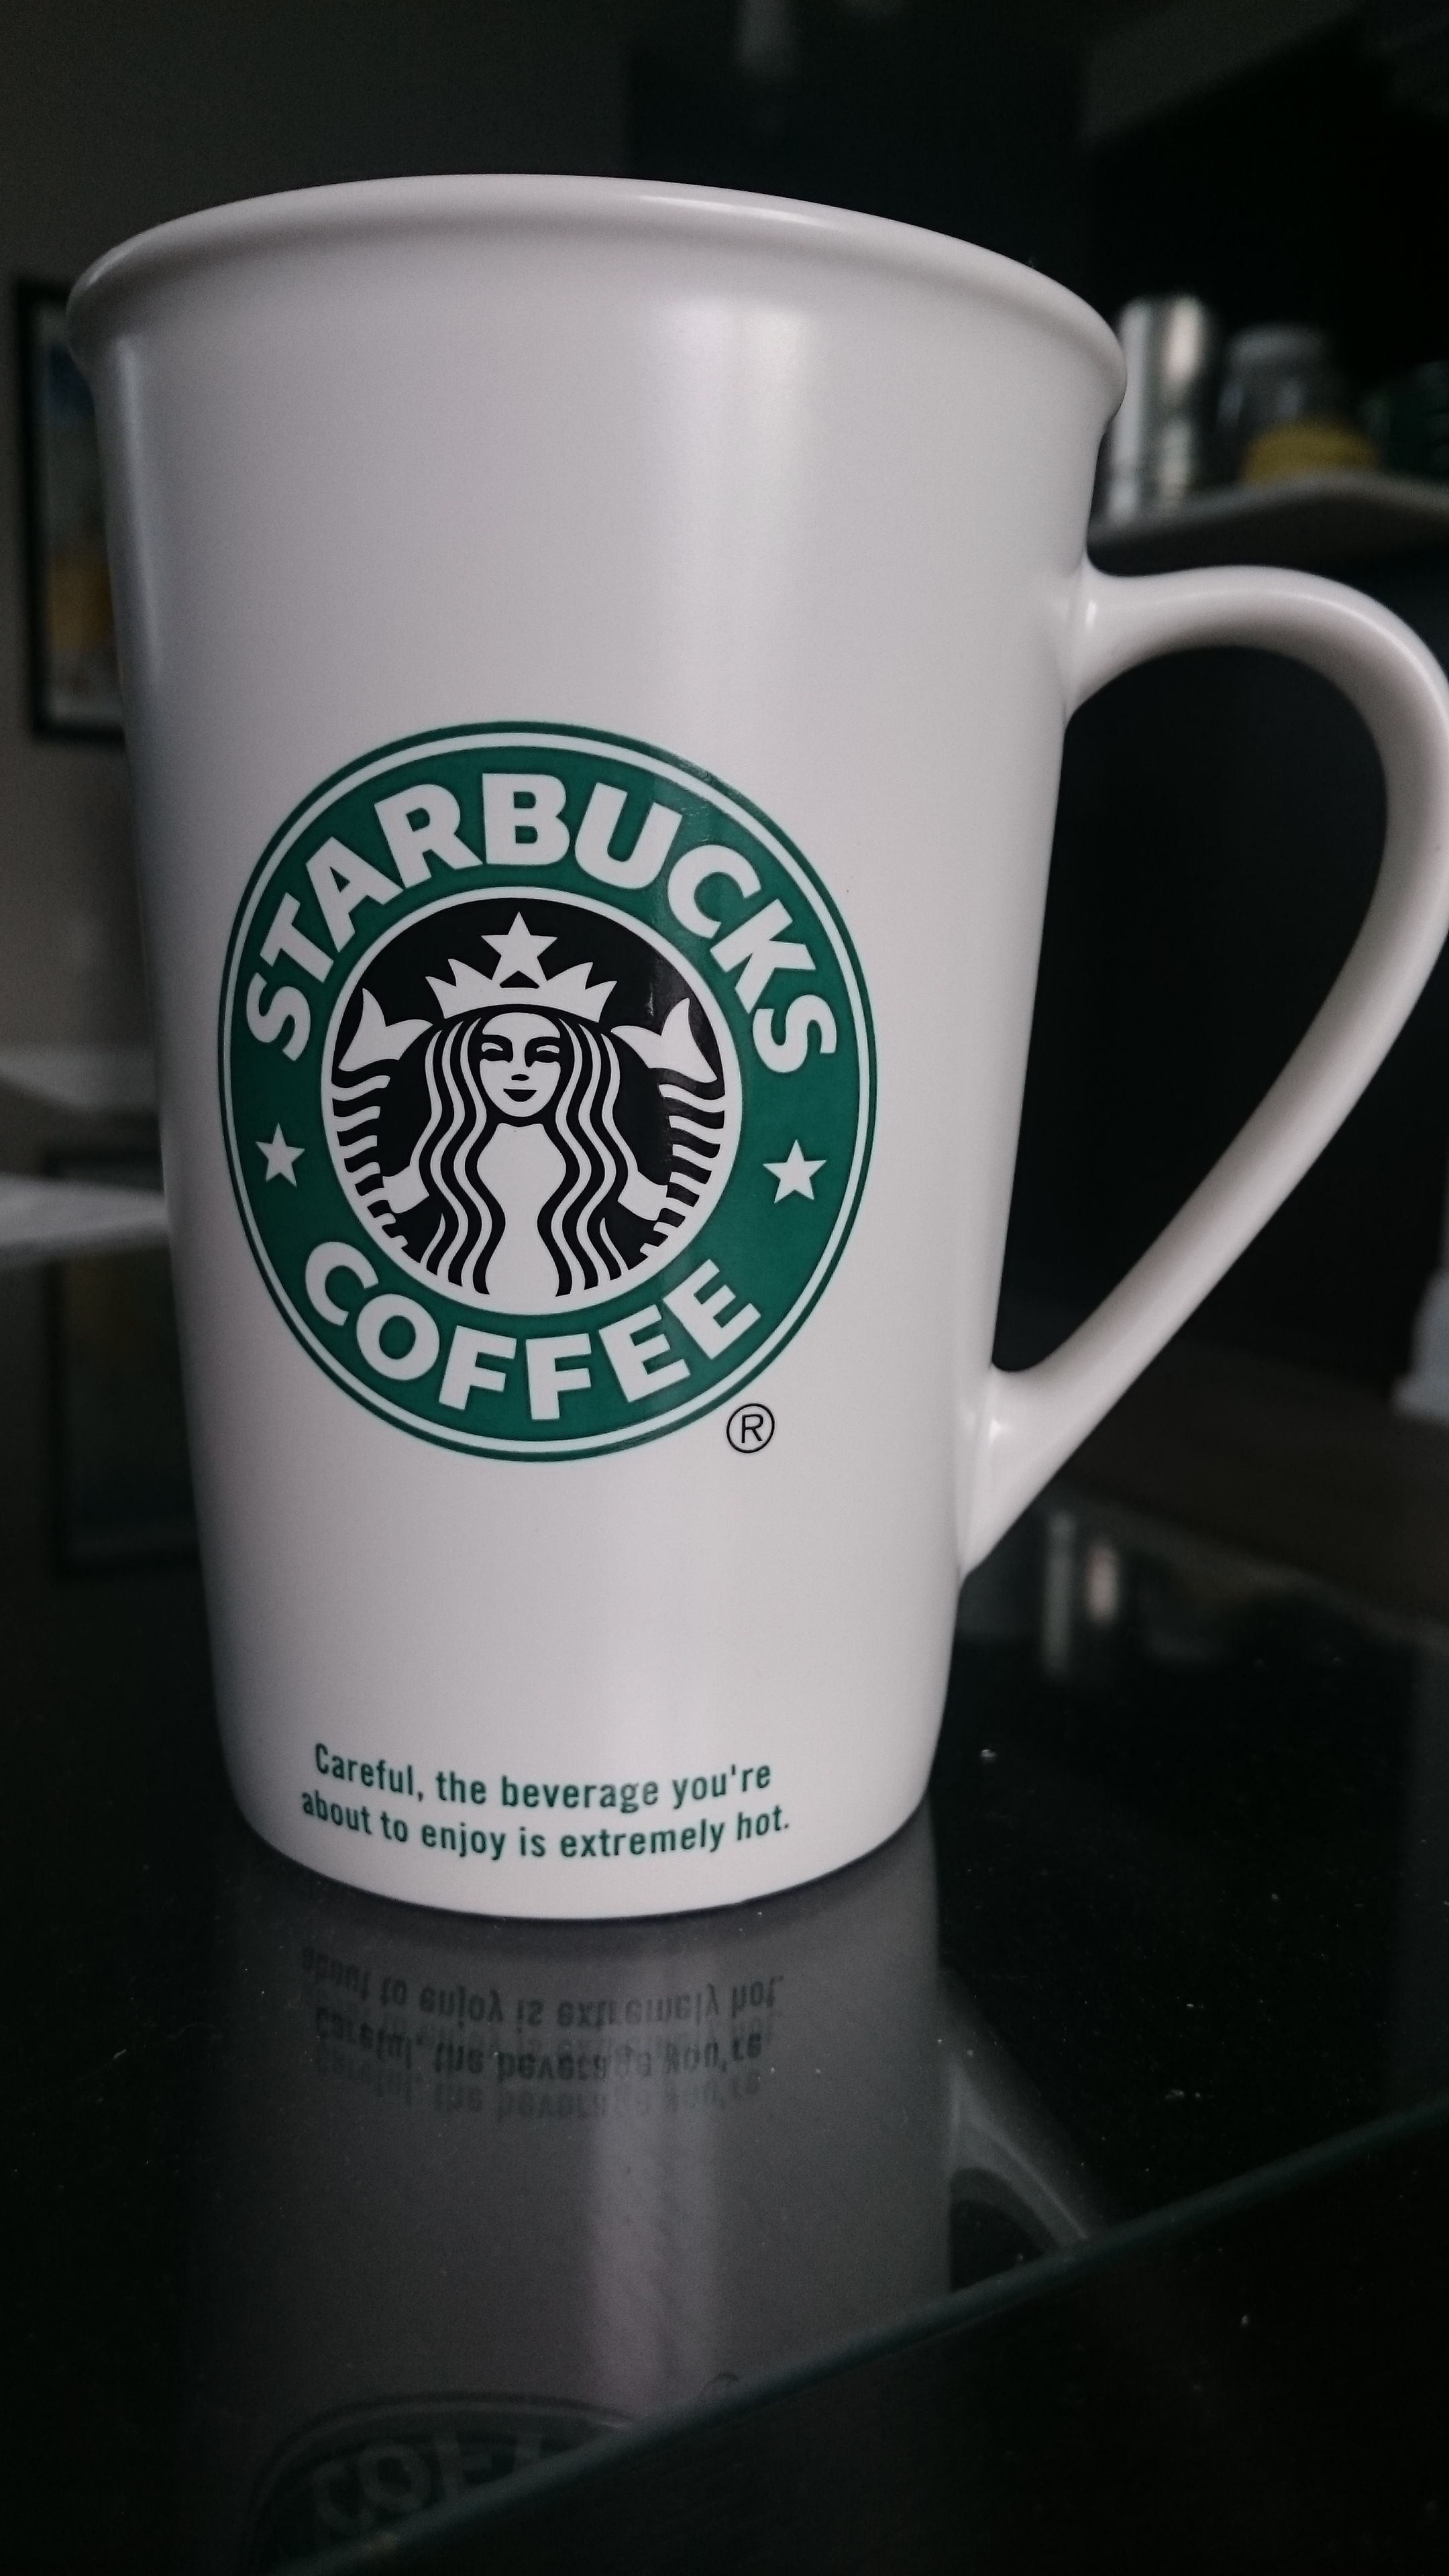
\includegraphics[width=0.5\textwidth]{images/coffeemug.jpg}
\end{center}

\end{frame}



\begin{frame}
\frametitle{Duty to Warn}

Manufacturers, sellers, distributors, et cetera, have a duty to warn consumers or users of any dangerous potential of a product.

On the basis of ``better safe than sorry'', you see warnings that coffee might be hot or that silica gel should not be eaten.

Labelling and warning signs are therefore tremendously common.

\end{frame}




\begin{frame}
\frametitle{Boom Goes the ... Shell?}

1976 case: \textit{George Ho Lem v. Barotto Sports Ltd. and Ponseness-Warren Inc.}~\cite{lpe}

The plaintiff purchased a shot-shell reloading machine that was not defective.\\
\quad If operated correctly, it would produce normal shot shells.

The plaintiff received instruction on how to use the machine as well as an instruction manual. He did not follow the instructions.

Misuse of the machine resulted in some dangerous shells; one caused an explosion in the chamber of the gun on firing and the plaintiff was injured.

\end{frame}



\begin{frame}
\frametitle{Exploding Shell}

The reloading machine was manufactured by one of the defendants and sold to the plaintiff by another.

The plaintiff claimed that they had not adequately warned him of the danger of a shell that was dangerous.

A shell with this defect would not be, from its appearance, obviously dangerous.

Should the plaintiff succeed in this claim?

\end{frame}



\begin{frame}
\frametitle{Appellate Court}

The appellate court found that the plaintiff had received adequate instructions on and warnings about the use of the machine.

The plaintiff's failure to follow the clear instructions caused his injuries.

Even though the machine is inherently dangerous -- gunpowder is literally an explosive -- the manufacturer lived up to its responsibility to warn users.

\end{frame}



\begin{frame}
\frametitle{More Explosions than Mythbusters}

Another explosion, another case: \textit{Lambert v. Lastoplex Chemicals Co. Limited et~al} in 1971~\cite{lpe}.

The plaintiff was a consulting engineer (who graduated from mechanical engineering) purchased a lacquer sealer.

He intended to use it to seal a floor in a basement, in which nearby was the furnace and water heater, both of which had pilot lights.

Fumes or vapours from the sealant came in contact with the pilot light, leading to a fire and then an explosion, damaging the house and burning the plaintiff.

\end{frame}



\begin{frame}
\frametitle{More Explosions than Mythbusters}

Obviously, had there been no warning labels, this would be a slam dunk case.

The product had three separate warnings, including:

\begin{enumerate}
	\item Caution inflammable! Keep away from open flame!
	\item KEEP AWAY FROM FIRE, HEAT, AND OPEN FLAME LIGHTS
	\item CAUTION, INFLAMMABLE -- Do not use near open flame or while smoking.
\end{enumerate}

Were these warnings enough?

\end{frame}



\begin{frame}
\frametitle{More Explosions than Mythbusters}

Does it help you decide if a competitor's product says the following?

\begin{quote}
DANGER-FLAMMABLE, DO NOT SMOKE. ADEQUATE VENTILATION TO THE OUTSIDE MUST BE PROVIDED. ALL SPARK PRODUCING DEVICES AND OPEN FLAMES (FURNACES, ALL PILOT LIGHTS, SPARK-PRODUCING SWITCHES, ETC.), MUST BE ELIMINATED, IN OR NEAR WORKING AREA.
\end{quote}


\end{frame}

\begin{frame}
\frametitle{Engineer}

Another complicating factor -- the plaintiff in question was an engineer.

Does the fact that he was qualified with special knowledge affect the ruling?


\end{frame}

\begin{frame}
\frametitle{Engineer}

The Supreme Court ruling said:

\begin{quote}
What was relied on by the respondent as special knowledge was the fact that the male appellant had qualified as a professional engineer, he knew from his experience that a lacquer sealer was inflammable and gave off vapours, and hence knew that it was dangerous to work with the product near a flame. This, however, does not go far enough to warrant a conclusion that the respondent, having regard to the cautions on the labels, had discharged its duty to the male appellant.
\end{quote}

So the fact that he was an engineer did not mean the plaintiff was responsible for the negative outcome.

Back to the original question -- are the provided warnings enough?

\end{frame}

\begin{frame}
\frametitle{Not Enough}
The Supreme Court ruling said:

\begin{quote}
Manufacturers owe a duty to consumers of their products to see that there are no defects in manufacture which are likely to give rise to injury in the ordinary course of use. Their duty does not, however, end if the product, although suitable for the purpose for which it is manufactured and marketed, is at the same time dangerous to use; and if they are aware of its dangerous character they cannot, without more, pass the risk of injury to the consumer.

\end{quote}

\end{frame}

\begin{frame}
\frametitle{Not Enough}
The Supreme Court ruling said:

\begin{quote}
 A general warning, as for example, that the product is inflammable, will not suffice where the likelihood of fire may be increased according to the surroundings in which it may reasonably be expected that the product will be used. The required explicitness of the warning will, of course, vary with the danger likely to be encountered in the ordinary use of the product.
\end{quote}

The warnings were found not explicit enough about the degree of danger.

\end{frame}



\begin{frame}
\frametitle{Takeaways on Product Liability}

This case should make it clear just how important product warning labels and instructions are.

Thus far, the duty to warn has come into play where an injury has occurred, or obvious damage. 

What if the loss were purely economic?

\end{frame}




\begin{frame}
\frametitle{References \& Disclaimer}
\bibliographystyle{alphaurl}
\setbeamertemplate{bibliography item}{\insertbiblabel}
{\scriptsize
\bibliography{290}
}
\vfill

{\tiny Disclaimer: the material presented in these lectures slides is intended for use in the course ECE~290 at the University of Waterloo and should not be relied upon as legal advice. Any reliance on these course slides by any party for any other purpose are the responsibility of such parties.  The author(s) accept(s) no responsibility for damages, if any, suffered by any party as a result of decisions made or actions based on these course slides for any other purpose than that for which it was intended.\par}


\end{frame}


\end{document}

